\part{Finite state machines}
\frame{\partpage}

\begin{frame}{Finite state machines}
    \begin{itemize}
        \pause\item A \textbf{finite state machine (FSM)} consists of:
            \begin{itemize}
                \pause\item A set of \textbf{states}; and
                \pause\item \textbf{Transitions} between states
            \end{itemize}
        \pause\item At any given time, the FSM is in a \textbf{single state} 
        \pause\item \textbf{Inputs} or \textbf{events} (\textbf{percepts}) can cause the FSM to transition to a different state
        \pause\item Which state the FSM is in dictates what \textbf{actions} the agent takes
    \end{itemize}
\end{frame}

\begin{frame}{State transition diagrams}
    \begin{center}\scalebox{0.8}{
        \begin{tikzpicture}[->,>=stealth',shorten >=1pt,auto,node distance=5cm,
                            semithick]
            \node[initial,state] (A) {a state};
            \node[state] (B) [right of=A, align=center] {another\\state};

            \path (A) edge [bend left] node [above] {transition} (B)
                  (B) edge [bend left] node [below] {transition} (A)
                  (A) edge [loop above] node {loop} (A);
        \end{tikzpicture}
    }\end{center}
    \begin{itemize}
        \pause\item FSMs are often drawn as \textbf{state transition diagrams}
        \pause\item Reminiscent of \textbf{flowcharts} and certain types of \textbf{UML diagram} 
    \end{itemize}
\end{frame}

% \begin{frame}{FSMs for AI behaviour}
%     The next slide shows a simple FSM for the following AI behaviour, for an enemy NPC in a shooter game: \pause
%     \begin{itemize}
%         \item By default, patrol (e.g.\ along a preset route) \pause
%         \item If the player is spotted, attack them \pause
%         \item If the player is no longer visible, resume patrolling \pause
%         \item If you are low on health, run away and find a medikit. Then resume patrolling \pause
%         \item If you are low on ammo, run away and find ammo. Then resume patrolling 
%     \end{itemize}
% \end{frame}

% \begin{frame}
%     \begin{center}\scalebox{0.8}{
%         \begin{tikzpicture}[->,>=stealth',shorten >=1pt,auto,node distance=5cm,
%                             semithick]
%             \node[initial,state] (patrol) {patrol};
%             \node[state] (health) [above right of=patrol, align=center] {seek\\medikit};
%             \node[state] (ammo) [below right of=patrol, align=center] {seek\\ammo};
%             \node[state] (attack) [above right of=ammo] {attack};

%             \path (patrol) edge [bend left] node [below] {player visible} (attack)
%                   (attack) edge [bend left] node [above] {player not visible} (patrol)
%                   (attack) edge node [above right] {low health} (health)
%                   (attack) edge node {out of ammo} (ammo)
%                   (health) edge node [above left] {medikit found} (patrol)
%                   (ammo) edge node {ammo found} (patrol);
%         \end{tikzpicture}
%     }\end{center}
% \end{frame}

\begin{frame}{Other uses of FSMs}
    As well as AI behaviours, FSMs may also be used for: \pause
    \begin{itemize}
        \item Animation \pause
        \item UI menu systems \pause
        \item Dialogue trees \pause
        \item Token parsing \pause
        \item ...
    \end{itemize}
\end{frame}

\begin{frame}[fragile]{Implementing FSMs}
    \begin{itemize}
        \pause\item Implementation needs to keep track of current state,
            and execute some code dependent on the state
            (this code itself possibly changing the current state)
        \pause\item Most common approach: a big \lstinline{switch}--\lstinline{case} statement,
            with an \lstinline{enum} type for the state
        \pause\item Object-oriented approach: a \lstinline{State} class, which your FSM states inherit from
        \pause\item Functional approach: represent state by a function delegate
        \pause\item Coroutine approach: encode your FSM logic as a procedure which runs as a coroutine
            (requires either refactoring logic into structured loops, or using \lstinline{goto}...)
    \end{itemize}
\end{frame}

\begin{frame}{Hierarchical FSMs}
    \begin{center}
        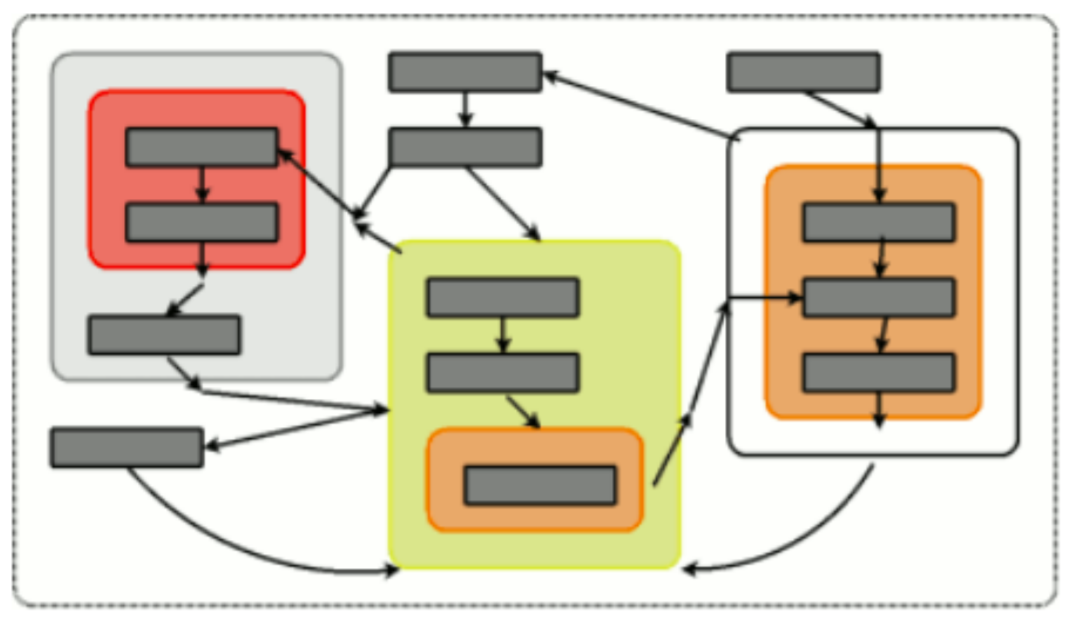
\includegraphics[width=0.7\textwidth]{hierarchical_fsm}
    \end{center}
    \begin{itemize}
        \pause\item An FSM with $N$ states has potentially $N^2$ transitions
        \pause\item Designing complex behaviour with FSMs quickly gets unwieldy
        \pause\item Hierarchical FSMs allow to group states into \textbf{super-states} to simplify defining transitions
    \end{itemize}
\end{frame}

\begin{frame}{Should you use FSMs?}
    \begin{itemize}
        \pause\item FSMs are useful for designing simple AI behaviours
        \pause\item Historically an important technique for game AI
        \pause\item However other techniques such as behaviour trees are more flexible
            and better suited to designing complex behaviours
    \end{itemize}
\end{frame}

